% =====================================================================
%  hc_leapfrog_v1.tex  --  Hydrocode sheet, Fig. 2: leapfrog timeline
%  CARTOON: one cycle, n -> n+1.  Velocity lives on half steps and is
%  advanced from n-1/2 to n+1/2 by the state at n; positions and density
%  then advance n -> n+1; energy, pressure, sound speed and q follow at
%  n+1.  Delta t^n is the interval from n to n+1.  No numbers.
% =====================================================================
\documentclass[tikz,border=6pt]{standalone}
\usepackage{amsmath,bm}
\usetikzlibrary{arrows.meta,decorations.pathreplacing}
\definecolor{slate}{HTML}{2C3E50}
\definecolor{oiblue}{HTML}{0072B2}
\definecolor{oiorange}{HTML}{E69F00}
\begin{document}
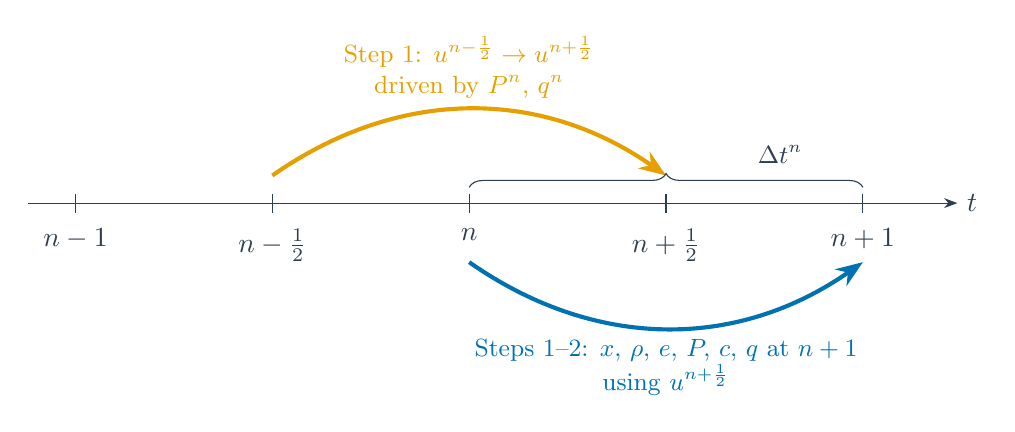
\begin{tikzpicture}[font=\sffamily, text=slate, >=Stealth]
  \draw[->,slate,thin] (-0.6,0) -- (11.2,0) node[right] {$t$};
  \foreach \x/\lab in {0/{n-1},2.5/{n-\frac{1}{2}},5/{n},7.5/{n+\frac{1}{2}},10/{n+1}} {
    \draw[slate] (\x,-0.12) -- (\x,0.12);
    \node[below=3pt] at (\x,-0.1) {$\lab$};
  }
  % velocity: half steps (above)
  \draw[->,oiorange,line width=1.5pt] (2.5,0.35) to[bend left=35]
     node[above,text=oiorange,font=\small,align=center] {Step 1: $u^{n-\frac{1}{2}} \rightarrow u^{n+\frac{1}{2}}$\\ driven by $P^n,\,q^n$} (7.5,0.35);
  % thermo: whole steps (below)
  \draw[->,oiblue,line width=1.5pt] (5,-0.75) to[bend right=35]
     node[below,text=oiblue,font=\small,align=center] {Steps 1--2: $x,\,\rho,\,e,\,P,\,c,\,q$ at $n+1$\\ using $u^{n+\frac{1}{2}}$} (10,-0.75);
  % dt brace
  \draw[decorate,decoration={brace,amplitude=5pt},slate] (5,0.2) -- (10,0.2);
  \node[font=\small] at (8.95,0.62) {$\Delta t^n$};
\end{tikzpicture}
\end{document}
